\documentclass{article}
\usepackage[b4paper]{geometry}
\usepackage[utf8]{inputenc}
\usepackage{breqn}
\usepackage{longtable}
\usepackage{graphicx}
\usepackage{tabularx}
\usepackage{caption}
\usepackage{graphicx}
\usepackage{float}
\usepackage[hidelinks]{hyperref}
\title{A quick report for model "mdl"}
\begin{document}
\maketitle


\section{Summary}


There are 1 repositary, 14 commodity, 6 technology, 2 supply, 1 demand.

\tableofcontents


\section{Commodity}


\subsection{COAL}


\begin{figure}[H]
  \centering
  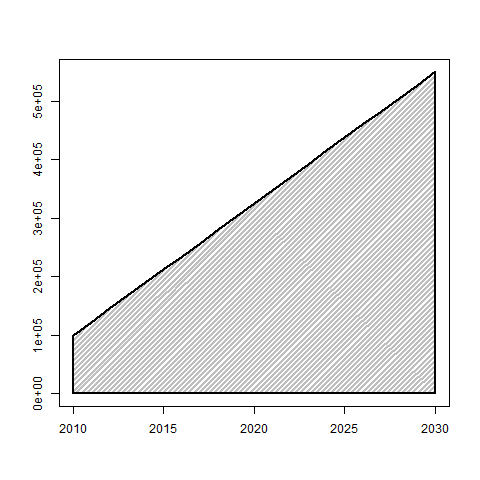
\includegraphics[width = 5in]{COAL_supply.png}
  \caption{Supply commodity COAL, summary for all region and slice.}
\end{figure}



\subsection{ELC}


\begin{figure}[H]
  \centering
  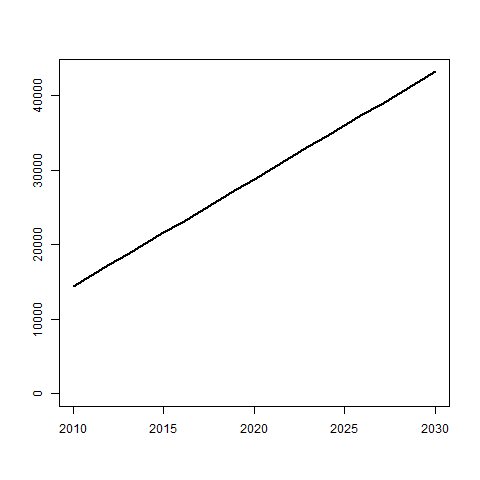
\includegraphics[width = 5in]{ELC_demand.png}
  \caption{Demand commodity ELC, summary for all region and slice.}
\end{figure}



